\section{Motivation}

\begin{frame}{Anonym?}
	\begin{figure}%[ht]
		\centering
		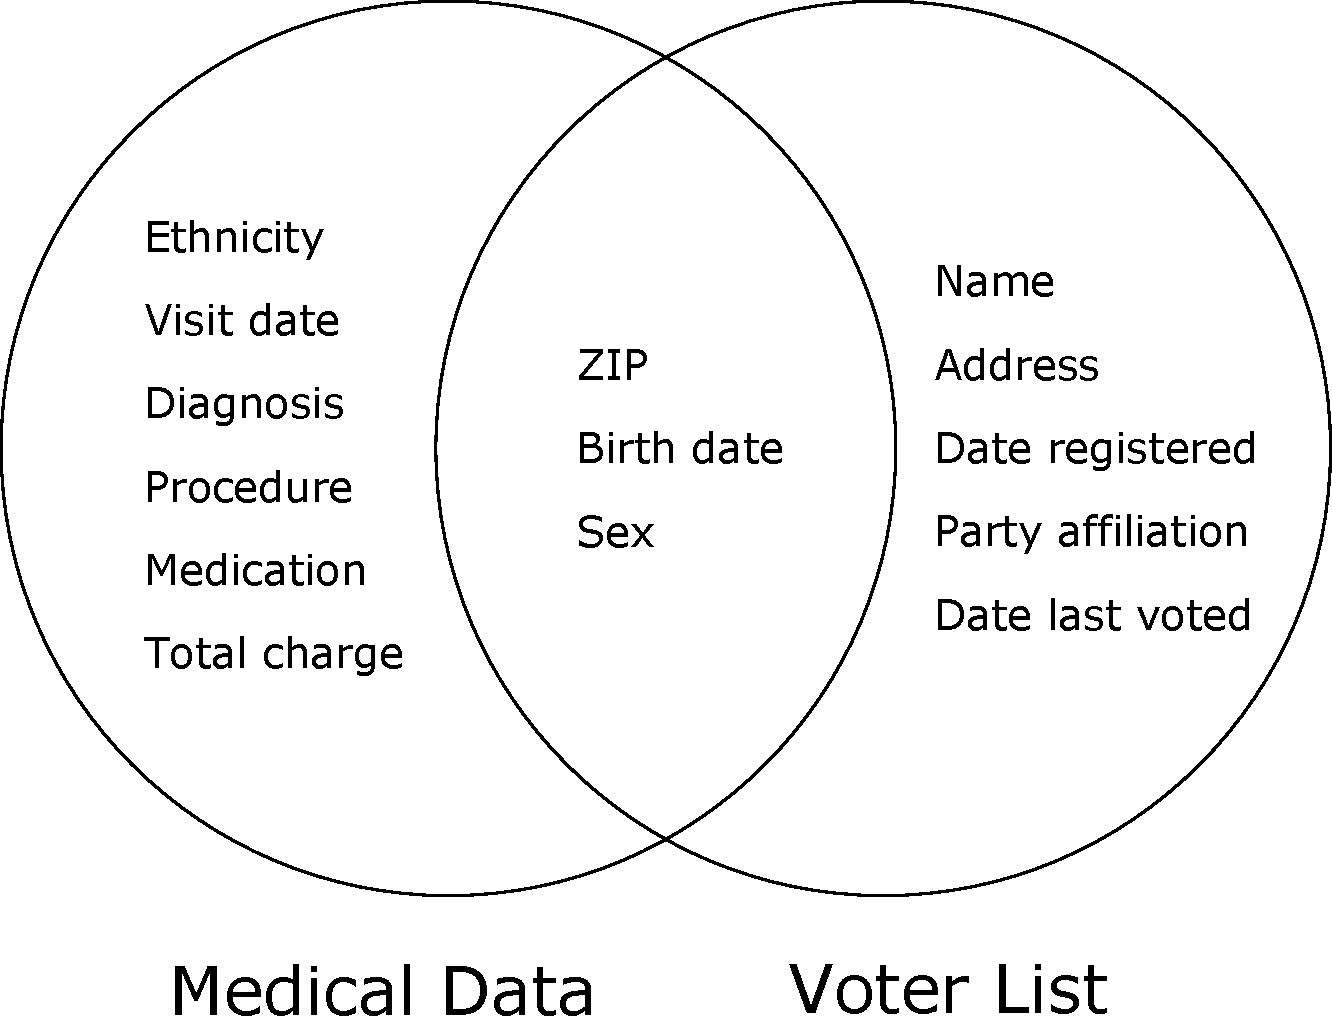
\includegraphics[width=0.7\textwidth]{pic/sweeney_governor.pdf}
		\vspace{0.2cm}
	
		\tiny Massachusetts Group Insurance Commission (GIC) medical data and voter registration data. Entnommen aus \cite{sweeney_k_anonymity}.
	\end{figure}

	%Sweeney - Beispiel \cite{sweeney_k_anonymity}
	%
	%---
	%
	%- Group Insurance Commission veröffentlichte Patientendaten in anonymer Form
	%
	%- Cambridge, Massachusetts voter registration list mit den öffentlichen Informationen der GIC abgeglichen
	%
	%- Beispielsweise konnte Massachusetts governor William Weld eindeutig identifiziert werden.
\end{frame}

\begin{frame}{Anonym? II}
	Sweeney \cite{sweeney_demographics}(1990) und Golle \cite{golle_demographics}(2000) überprüften die Eindeutigkeit von demographischen Faktoren in der Bevölkerung der USA.
	
	%	Sweeney für die 1990 US census data, Golle wiederholte das für 2000
	%
	%\begin{center}
	%	\begin{tabular}{|r|r|r|r|r|}
	%	\hline	 & \textbf{Geb.dat.} & \textbf{M. \& J.} & \textbf{J.} & \textbf{2 J.} \\
	%	\hline \textbf{PLZ} & 87.1 & 3.7 & 0.04 & 0.01 \\
	%	\hline \textbf{Ort} & 58.4 & 3.6 & 0.04 & 0.01 \\
	%	\hline \textbf{County} & 18.1 & 0.04 & 0.00004 & 0.00000 \\
	%	\hline
	%	\end{tabular}
	%\end{center}
	
	\begin{center}
		\begin{tabular}{|r|r|r|r|r|}
		\hline	 & \textbf{T. M. J.} & \textbf{M. J.} & \textbf{J.} & \textbf{2 J.} \\
		\hline \textbf{PLZ} & 87.1 \% & 3.7 \% & 0.04 \% & 0.01 \% \\
		\hline \textbf{Ort} & 58.4 \% & 3.6 \% & 0.04 \% & 0.01 \% \\
		\hline \textbf{County} & 18.1 \% & 0.04 \% & 0.00004 \% & 0.00000 \% \\
		\hline
		\end{tabular}
		\vspace{0.2cm}
	
		\tiny Eindeutig identifizierbarer Individuenanteil an der U.S.-Bevölkerung 1990. Entnommen aus \cite{sweeney_demographics}.
	\end{center}

	\textbf{Ergebnis}: Durch \{Geburtsdatum, Geschlecht, PLZ\} könnten \textasciitilde{}87\% der Bevölkerung eindeutig identifiziert werden.
		
	%	
	%	---
	%	
	%	Basierend auf den Daten, die folgende Felder darstellen (aggregiert): 
	%	
	%	StateID 	State Code 
	%	ZIP 		5-digit ZIP 
	%	TotPop 		Total Population 
	%	AUnder12 	Population Under Age 12 Years 
	%	A12to18 	Population Age 12-18 Years 
	%	A19to24 	Population Age 19-24 Years 
	%	A25to34 	Population Age 25-34 Years 
	%	A35to44 	Population Age 35-44 Years 
	%	A45to54 	Population Age 45-54 Years 
	%	A55to64 	Population Age 55-64 Years 
	%	A65Plus 	Population Age 65 Years and up 
	%	
	%	Betrachtet wird jeweils die Anzahl unterschiedlicher möglicher unterschiedlicher Werte, die sich für die entsprechenden Attribute ergeben und die tatsächliche Anzahl der Population. Wenn die Anzahl möglicher Ausprägungen die tatsächliche Population übertrifft, dann werden die Individuen als eindeutig identifizierbar angesehen, ansonsten nicht -> Grobe Abschätzung.
\end{frame}

\begin{frame}{Abgrenzung}
	\begin{center}
		Vermeintlich anonyme Daten stellen sich als nicht anonym heraus. \textbf{Daher}: Wie können wir Aussagen über die "'Güte"' der Anonymisierung machen?
	\end{center}

	\vspace{0.5cm}
	\pause
	
	Worum es nicht gehen soll:
	
	\begin{itemize}
		\item Begrenzung des Zugriffs (Authentifikation, Multi-Level-Datenbanken)
		\item Statistische Datenbanken (Aggregation, Begrenzung von Selektionsarten, Logging und Abwägen von Anfragen, Hinzufügen von Zufall)
	\end{itemize}
	
	Darum geht es:
	
	\begin{itemize}
		\item Veröffentlichung von Daten als Individualdatensätze ohne Integritätsverlust unter Wahrung der Anonymität.
	\end{itemize}
\end{frame}
